\subsection{Tipi fondamentali}
In \code{C++} abbiamo dei \textbf{tipi fondamentali}, che sono implementati di base dal linguaggio. Si chiamano \textbf{Built-in(integrati)}\newline
questi tipi sono: 
\begin{itemize}
    \item \textbf{\textcolor{blue}{Built-in (Integrati)}:}
        \begin{itemize}
            \item \code{\textbf{Boolean}}
            \item \code{\textbf{char}}
            \item \code{\textbf{int} , long int, long long int...}
            \item \code{float , \textbf{double}, long double}
            \item \textbf{void}
            \item \textbf{Puntatori(es: \code{int*})}, \textbf{Array} e \textbf{Riferimenti(\code{double\&})}
        \end{itemize}
    \item \textbf{\textcolor{blue}{User-defined}:}
        \begin{itemize}
            \item enum
            \item \textbf{classes}
            \item \textbf{tipi introdotti dalle librerie standard}
        \end{itemize}
\end{itemize}
Un \textbf{'\code{tipo}'} serve per definire il \textbf{dominio} dei valori che può assumere quel elemento. Il \textbf{'\code{tipo}'} serve anche per definire l'insieme di \textbf{operazioni} che si possono essere fate su quel tipo. \newline\newline
poi intendiamo come \textbf{letterale} tutti i valori inseriti direttamente nel codice
\lstinputlisting{Capitoli/Tipi di dato/Esempi/Esletterali.txt}

\newpage
\subsubsection{Sizeof()}
Il \code{Sizeof()} permette di controllare lo spazio che occupa un determinato tipo o variabile. Il peso dei tipi va in base all'implementazione del programmatore. Quindi il programmatore può modificare le grandezze di default.
questo può comportare dei vantaggi e dei svantaggi.\newline\newline
 \textbf{\textcolor{blue}{Vantaggi:}}
\begin{itemize}
    \item Utilizzando grandezze personalizzate posso sfruttare a meglio il mio hardware(memoria)\newline
\end{itemize}
\textbf{\textcolor{blue}{Svantaggi:}}
\begin{itemize}
    \item Il codice diventa meno portatile poiché diventerebbe più specifico per un certo hardware(meno portatile)
    \item rischio che con le versioni future del compilatore non potrebbe funzionare poiché si sono modificati valori di default
\end{itemize}

Quindi dobbiamo modificare questi valori solo quando è veramente necessario poiché a noi ci interessa la portabilità del codice

\subsection{Inizializzazioni}
\hypertarget{init}{}
Possiamo inizializzare una variabile in 4 modi:

\begin{enumerate}
    \item Graffe(list initialization): \code{int a1 \{15\}};
    \item Uguale + graffe: \code{int a2 = \{15\};}
    \item Uguale: \code{ int a3 = 15;}
    \item Tonde:  \code{int a4(15);}
\end{enumerate}
\textbf{\textcolor{blue}{Cosa utilizzare?}}
\begin{itemize}
    \item La prima forma è \textbf{PREFERIBILE} poiché controlla che varie conversioni non perdano informazioni.
    \item Se non viene inserito nessun valore viene inizializzato a un valore di default, questo metodo di inizializzazione e più leggibile e permette meno errori.
    \lstinputlisting{Capitoli/Tipi di dato/Esempi/InParentesigraffeEs.txt}
\end{itemize}
Possiamo inizializzare anche una lista di elementi:
\lstinputlisting{Capitoli/Tipi di dato/Esempi/vettoreIn.txt}

\subsection{Tipo Booleano}
Il tipo booleano può essere solo due valori \textcolor{blue}{\code{True}} o \textcolor{blue}{\code{False}}.\newline Possiamo subito dire che: 
\begin{itemize}
    \item Un qualsiasi valore intero diverso da zero è convertito in booleano come  \textcolor{blue}{\code{True}}, altrimenti un valore uguale a zero come  \textcolor{blue}{\code{False}}
    \lstinputlisting{Capitoli/Tipi di dato/Esempi/EsempioconversioneBool.txt}
    \item Un puntatore può essere convertito \code{True} se punta a qualcosa , altrimenti se non punta a nulla(\code{nullptr}) a \code{false}
\end{itemize}

\subsection{Tipo carattere}
Esistono vari tipi di caratteri (come i latini o gli ideogrammi cinesi ecc.) ognuno di essi ha la sua propia codifica.\newline\newline
Ovviamente non esiste solo il tipo \code{char}, Esistono numerosi tipi che supportano anche diversi tipi di codifica. nella maggior parte dei casi basta il \code{char} con i suoi \code{8 bits}. \newline\newline
Il \code{char} supporta la codifica ASCII ed è in grado di immagazzinare un solo carattere (1 Byte). \newline\newline
Esistono anche dei caratteri speciali che utilizzano il carattere " \textbackslash " come "\textbackslash n".
\newpage
\subsection{Tipo Intero}
Abbiamo diversi tipi di intero:
\begin{itemize}
    \item Con il segno(\code{unsigned})
    \item Diverse dimensioni(\code{int , short int , long int ecc.})
\end{itemize}
\begin{itemize}
    \item utilizzare \code{unsigned} per risparmiare \code{1 bit} non ha senso, è quasi in rilevante in vasta scala.
    \item \textbf{letterali} sono interi e tutti espressi in decimale , esadecimale , ottale(es: base 10(1), base 16(0x1) , base 8(01))
    \item Il tipo di ogni letterale è deciso dal suo suffisso, se c’è (ad
    esempio: u o U per \code{usigned}, l o L for \code{long}, ll o LL for \code{long long}) e dal tipo di lunghezza minima che ne contiene il
    valore.

\end{itemize}


\subsection{Tipo virgola mobile (floating point)}
\begin{itemize}
    \item \code{double} è il \textbf{default}. Quindi il tipo base per esprimere numeri con la virgola.
    \item I Sono letterali validi: 1.23, .23, -2.3, 0.23, 1., 1.0, 1.2e10,
    1.23e-15 (niente spazi attorno alla e)
    \item Suffisso f se voglio che sia un \code{float (2.0f)}
    \item Suffisso L per \code{long double}.
\end{itemize}

\subsection{Tipo void}
\begin{itemize}
    \item  Non possono esistere oggetti di tipo void.
    
    \item Si usa solo in due casi:
        \begin{enumerate}
            \item Per indicare che una funzione non restituisce nulla;
            \item Per indicare il tipo di un puntatore ad un oggetto di tipo
            sconosciuto
        \end{enumerate}
\end{itemize}
\newpage
\subsection{Tipo costante}
\textbf{\textcolor{blue}{\code{const}}}: “Prometto di non cambiare questo valore” e il compilatore controlla che sia proprio così. \newline
\textbf{\textcolor{blue}{\code{constexpr }}}: “Da valutare a tempo di compilazione”.
Possono essere \code{constexpr} anche funzioni, ma solo se
molto semplici (solo un’istruzione di \code{return})\newline
Distinzione sottile, che per il momento potete non
considerare

\subsection{Tipo punatore e riferimento}
\begin{itemize}
    \item Possiamo accedere a una variabile nei seguenti modi:
    \begin{itemize}
        \item usando il nome
        \item dal suo indirizzo di memoria, tenendo conto del tipo della
        variabile
        \item dal suo riferimento
    \end{itemize}
    \item Puntatori e riferimenti servono esattamente a questo, in
    due modi leggermente diversi.
\end{itemize}
 Esempio di puntatore:
 \lstinputlisting{Capitoli/Tipi di dato/Esempi/EsPtr.txt}
 \begin{center}
     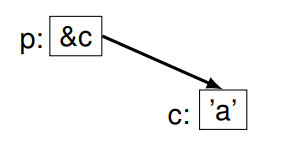
\includegraphics[scale = 0.6]{Capitoli/Tipi di dato/Esempi/ptr.png}
 \end{center}
 \begin{itemize}
     \item \code{c2} assume il valore puntato da \code{p}, nel senso che \code{c2} assume il valore memorizzato all’indirizzo contenuto in \code{p}
    \item quindi: la memoria viene letta sapendo il tipo della
    variabile, altrimenti sarebbe impossibile.
    \item L’oggetto puntato da \code{p} è \code{c}, il cui valore è \code{’a’}
    \item in conclusione: \code{c2} assume il valore del letterale \code{’a’}
 \end{itemize}
Quando accediamo a un valore puntato da un puntatore(quindi trmite l'Indirizzo contenuto nel puntatore) stiamo effettuando la differenziazione tramite l'operatore unario \textcolor{blue}{\code{*}}.\newline\newline
I puntatori hanno una aritmetica chiamata \textbf{aritmetica dei puntatori} che utilizza l'indirizzamento della memoria. Ci permette di lavorare sugli indirizzi facendo delle operazioni(es: sommare un valore a un indirizzo) su questi indirizzi. Questa indirizzazione avviene tramite \textbf{bytes}.\newline\newline
Quindi il più piccolo oggetto che può venir allocato e
indirizzato indipendentemente è il \code{char}, che corrisponde
ad un byte. infatti il \code{bool} occupa almeno tanta memoria quanto un \code{char}.\newline\newline
Ottimo se ho bisogno di implementare applicazioni che
scendano a quel livello di dettaglio (ad esempio, un
sistema operativo) \newline Se invece voglio fare una buona applicazione portabile,
meglio non usare queste operazioni di basso livello.\newline\newline\newline
\textbf{Per trasformare} un qualsiasi tipo \code{X} nel
corrispondente puntatore a \code{X} dobbiamo aggiungere al tipo
il suffisso \code{*}\newline\newline
\lstinputlisting{Capitoli/Tipi di dato/Esempi/EsPtr2.txt}
\textbf{Invece per le funzioni:}
\lstinputlisting{Capitoli/Tipi di dato/Esempi/EsPtr3Funz.txt}
\newpage 
\subsubsection{Puntatori a void}
\begin{itemize}
    \item Se dichiariamo una variabile di tipo \code{void*}, le possiamo
    assegnare un puntatore ad un qualsiasi tipo di oggetto.
    \item Possiamo considerarlo un \textbf{puntatore ad un oggetto di
    tipo sconosciuto}
    \item \textbf{Però} non può essere né un puntatore a funzione né un
    puntatore a un membro di una classe (inclusi i membri
    funzione o metodi)
    \item Se ho due variabili di tipo \code{void*}, posso:
    \begin{itemize}
        \item assegnare il valore dell’una all’altra
        \item confrontarle (sia eguaglianza che diseguaglianza)
        \item posso convertirle \textbf{esplicitamente} ad un altro tipo \end{itemize}
    \item Qualsiasi altra operazione può essere \textbf{pericolosa} e quindi
    va evitata: dà \textbf{errore} a tempo di compilazione
    \item Per usare un \code{void*} dobbiamo convertirlo esplicitamente
    ad un puntatore di un dato tipo
    \lstinputlisting{Capitoli/Tipi di dato/Esempi/EsPtrVoid.txt}
\end{itemize}
\code{int* pi2 = static\_cast<int*>(pv);}\newline dove \code{static\_cast<int*>} è un cast statico , questo cast aviene durante la compilazione e non durate il run-time
\begin{itemize}
    \item In genere, usare un puntatore ad un tipo \code{X1} per puntare ad  un oggetto di tipo \code{X2} è pericoloso(es: Il codi qui sopra). quindi usare il "cast" potrebbe creare problemi
    \item Pensiamo ad esempio che la dimensione di un oggetto
    può dipendere dall’implementazione . . .
    \item Cerchiamo quindi di usare questo operatore il meno
    possibile
    \item Il puntatore \code{void*} si usa per operazioni a basso livello sulla memoria
    \item In questi casi, gli usi più diffusi di \code{void*} sono:
    \begin{itemize}
        \item voglio passare un parametro ad una funzione senza fare
        ipotesi sul tipo dell’oggetto puntato
        \item la funzione deve tornare un puntatore ma senza fare ipotesi sul tipo dell’oggetto puntato
    \end{itemize}
    
    \item Se l’operazione è a più alto livello, meglio utilizzare
    soluzioni basate su un progetto orientato agli oggetti

\end{itemize}

\subsubsection{nullptr}
Letterale che rappresenta il \textbf{puntatore nullo}, ovvero il
puntatore che non punta a nessun oggetto
I Può venir assegnato a qualsiasi tipo di puntatore, ma non
agli altri tipi \textcolor{blue}{built-in}:
\lstinputlisting{Capitoli/Tipi di dato/Esempi/Esnullptr.txt}
 Un unico \code{nullptr} per qualsiasi tipo di puntatore
 \begin{itemize}
    \item Nessun oggetto può venir allocato all’indirizzo 0 (ovvero il
    pattern con tutti i bit a zero), quindi una volta si usava
    l’intero 0 al posto del puntatore nullo
    \item Addirittura si definiva una macro \code{NULL} per rappresentare il
    puntatore \code{null}
    \item Tuttavia
    \begin{itemize}
        \item la definizione di \code{NULL} dipende dall’implementazione (ad esempio, può essere 0 o 0L)
        \item la definizione usata in \code{C} (\code{(void*)0}) è illegale in \code{C++}
    \end{itemize}
    \item Conclusione: usate \code{nullptr}!

 \end{itemize}
\newpage

 \subsection{Array}
 \begin{itemize}
    \item Un array è una raccolta di dati di tipi omogenei fra di loro.
    \item Un array di Tipo \textcolor{blue}{\textbf{\code{X}}} deve essere indicato nel seguente modo se è definito in modo statico \textcolor{blue}{\textbf{\code{X NomeArray[size]}}}.
    l'indice va da \code{0} (index 0) fino a \code{size-1}(index -1)
     \lstinputlisting{Capitoli/Tipi di dato/Esempi/EsArray.txt}
    \item Possiamo usare l'operatore \textcolor{blue}{\code{[]}} per accedere oppure l'operatore unario \textcolor{blue}{\code{*}} (preferibile \textcolor{blue}{\code{[]}} poiché \textcolor{blue}{\code{*}} lavora troppo a basso livello)
    \item andare oltre alla lunghezza del array ha un comportamento indefinito e disastroso poiché non si sa cosa c'è dopo.
    \item quando inizializziamo un array la grandezza (\textcolor{blue}{\code{size}}) deve essere ben definita cioè un letterale. altrimenti il comportamento è indefinito. 
    \item possiamo invece usare il \textbf{\textcolor{blue}{\code{Vector}}} all'interno della standard library. a differenza del array conserverà la sua grandezza e quindi può essere definita come una variabile.
    \lstinputlisting{Capitoli/Tipi di dato/Esempi/EsArray2.txt}
 \end{itemize}
\textbf{\textcolor{blue}{Limitazioni Array built-in:}}
\begin{itemize}
    \item Si tratta di una struttura inerentemente di \textbf{basso livello}, da usarsi essenzialmente per costruire strutture di più \textbf{alto
    livello}, quali le strutture \textbf{vector} e \textbf{array} della libreria standard.
    \begin{itemize}
        \item  Non è possibile assegnare un \textbf{array} ad un altro \textbf{array}. Questo a meno che \textbf{l'array} destinazione non sia un puntatore a il tipo del \textbf{array} che dovrà essere assegnato.
        \lstinputlisting{Capitoli/Tipi di dato/Esempi/EsArray3.txt}
        \item  Come conseguenza, non è possibile passare un \textbf{array} ad
        una funzione per valore(altrimenti  si dovrebbe copiare l'intero \textbf{array}).
        \item  Il nome di un \textbf{array} viene implicitamente convertito ad un puntatore al suo primo elemento in molti contesti (poi
        vediamo meglio)
    \end{itemize}
    
    \item  Uno degli \textbf{array} più utilizzati è \textbf{l’array} di \code{char} terminato dal \code{char \textbackslash0}: una stringa in stile C: conservata per compatibilità con librerie già esistenti.

\end{itemize}


\subsubsection{Inizializzazione Array}
Possiamo inizializzare un Array in diversi modi:
\lstinputlisting{Capitoli/Tipi di dato/Esempi/InitArrayes.txt}
\begin{itemize}
    \item Nel caso in cui specifichiamo la dimensione e non inseriremo abbastanza elementi durante la inizializzazione allora saranno impostati a zero.
    \item Se non definiamo il numero di elementi che conterrà un array ma definiamo qual'è elemento ci dovrà essere allora il compilatore capirà da solo quanto spazzino allocare.
\end{itemize}
\subsubsection{Letterali stringa}
Un letterale stringa è un tipo costante (\code{const char}). Ogni letterale finisce con \code{'\textbackslash 0'}. \newline
Ogni carattere occupa \code{1 byte} quindi un letterale con 5 caratteri sarà un \newline\code{const char[5]}
\begin{itemize}
    \item \textbf{letterali stringa sono costanti, quindi immutabili}.
    \item  Se vogliamo usarla come inizializzazione e poi modificarla,
    dobbiamo usare l’array di caratteri (non costante):
    \lstinputlisting{Capitoli/Tipi di dato/Esempi/EsletString.txt}
    \item letterali stringa sono \textbf{allocati staticamente}, quindi possono essere restituiti da funzioni in modo sicuro. Poiché dopo alla chiamata di funzione la stringa è allocata in modo statico non sarà persa.
    
    \lstinputlisting{Capitoli/Tipi di dato/Esempi/EsritString.txt}
    \item Il codice viene \textbf{ottimizzato}, quindi in alcuni casi può
    succedere che due letterali stringa identici non vengano
    duplicati. quindi viene usato lo stesso letterale.
    \item Questo significa che non possiamo ipotizzare con certezza
    cosa succede.
    \lstinputlisting{Capitoli/Tipi di dato/Esempi/EsotString.txt}
    \item L’espressione \textcolor{blue}{\code{p==q}} confronta gli indirizzi, cioè i valori
    dei puntatori e non degli oggetti puntati.
    \item La lista vuota è \code{""}, ha tipo \code{const char[1]} e contiene il
    solo carattere \code{’\textbackslash 0’}.
    \item Per rappresentare i caratteri non grafici all’interno di una
    stringa possiamo utilizzare il \code{\textbackslash}:\newline
    \code{cout << "beep at end of message\textbackslash a\textbackslash n";}\newline
    \item Un problema possono essere le stringhe contenenti il
    carattere nullo
    \begin{itemize}
        \item  Sono perfettamente legali.
        \item La maggior parte dei programmi considererà solo la parte
        prima del primo carattere nullo: \code{Jens\textbackslash000Munk} verrà considerato come \code{"Jens"}.
        
    \end{itemize}
    \item  Il carattere di \textbf{newline} non può essere incluso in una
    stringa: una stringa non può stare su più righe. Devo
    invece usare \code{’\textbackslash n’}
    \item Se una stringa è troppo lunga può essere spezzata
    \lstinputlisting{Capitoli/Tipi di dato/Esempi/SpezString.txt}
\end{itemize}
\newpage
\subsubsection{Array come puntatore}
\begin{itemize}
    \item Legame stretto tra array e puntatori: il nome di un array
    può venir utilizzato come \textbf{puntatore al suo primo elemento}.
    \lstinputlisting{Capitoli/Tipi di dato/Esempi/EsPtrArray.txt}
    \begin{center}
        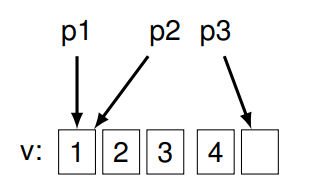
\includegraphics[scale = 0.6]{Capitoli/Tipi di dato/Esempi/EsPtrArray.png}
    \end{center}
    \item \textbf{Puntare} ad un elemento immediatamente successivo alla
    fine dell’array non dà errore, purché non si legga o scriva.
    \item Quando passiamo un \code{array} come parametro non ci sarà modo di passare una copia. sarà sempre passato il \textbf{riferimento} , questa conversione implicita da \textcolor{blue}{\code{array}} a  \textcolor{blue}{\code{puntatore}} farà perdere la grandezza del \code{array}.
    quindi non ci sarà modo di evitare questa conversione implicita.
    \lstinputlisting{Capitoli/Tipi di      dato/Esempi/EsempiArrayDopoSize.txt}
\end{itemize}
\newpage
\subsubsection{Navigazioni degli Array}
Abbiamo due modi per navigare in un array:
\begin{itemize}
    \item Utilizzare l'operatore \textcolor{blue}{\code{*}}. quindi sommare al indirizzo del \code{array} \textbf{l'indice} che vogliamo raggiungere e poi fare la Dereferenziazione per ottenere il contenuto.
    \item Utilizzare le \textbf{parenesi quadrate} con al interno l'indice
    \item \textbf{nessuna delle due e più efficiente del altra}, per una questione di leggibilità e meglio con le parentesi quadrate.
    \lstinputlisting{Capitoli/Tipi di dato/Esempi/NavigazioneArray.txt}
\end{itemize}

\subsubsection{Array Multidimensionali e Array come argomento di funzione}
\begin{itemize}
    \item Gli array multidimensionali sono rappresentati come array
    di array
    \item I Esempio 3x5:
    \lstinputlisting{Capitoli/Tipi di dato/Esempi/Matrix.txt}
    \item  Come per gli \code{array} ad una sola dimensione, le
    dimensioni non sono memorizzate in alcun modo nella
    struttura dati \code{array}
    \item Un array non può venir passato ad una funzione per
    valore, ma con un puntatore al suo primo elemento
    \lstinputlisting{Capitoli/Tipi di dato/Esempi/PassaggioArrayPar.txt}
\end{itemize}

\subsection{Riferimenti}
\begin{itemize}
    \item  \textbf{Un riferimento} (reference) può essere visto come un nome
    alternativo per un oggetto, un alias.
    \item \textcolor{blue}{\textbf{Analogamente ai puntatori:}}
    \begin{itemize}
        \item è un alias per un oggetto
        \item è implementato per conservare l’indirizzo di un oggetto
        \item non richiede maggiori risorse computazionali
    \end{itemize}

    \item \textcolor{blue}{\textbf{Diversamente dai puntatori, il riferimento:}}
    \begin{itemize}
        \item la sintassi è la stessa che avrei col nome dell'oggetto
        \item si riferisce sempre all'oggetto con cui è stata inizializzata
        \item \textbf{non esiste un “riferimento null”} da controllare: ogni
        riferimento si riferisce ad un oggetto
        \lstinputlisting{Capitoli/Tipi di dato/Esempi/EsempioReferance.txt}
    \end{itemize}
    \item Tra i \textbf{vantaggi} dei puntatori c’è quello di poter passare ad
    esempio ad una funzione una grande quantità di dati a
    basso costo.
    \item Però un puntatore ha una sintassi un po’ pesante . . .
    \item e può cambiare valore nel tempo, Invece il \textbf{riferimento} si riferirà \textbf{\textcolor{blue}{SEMPRE}} al oggetto a cui è stato inizializzato
    \item Inoltre bisogna sempre gestire la possibilità che il
    puntatore non stia puntando a nulla \textbf{(nullptr)}.
    \item Coi riferimenti non ho questi problemi.

\end{itemize}


